% Define professional, publication-friendly colors
\definecolor{decreasecolor}{RGB}{40, 167, 69} % A nice, clear green
\definecolor{increasecolor}{RGB}{220, 53, 69} % A corresponding clear red

\newcommand{\up}{\textcolor{increasecolor}{$\uparrow$}}
\newcommand{\down}{\textcolor{decreasecolor}{$\downarrow$}}
\newcommand{\phup}{\phantom{$\uparrow$}}
\newcommand{\phdown}{\phantom{$\downarrow$}}


\subsection{Analysis of Model Scales Generalizability}
\label{sec:scaling_analysis}


\begin{wrapfigure}{!r}{0.6\textwidth}
    \centering
    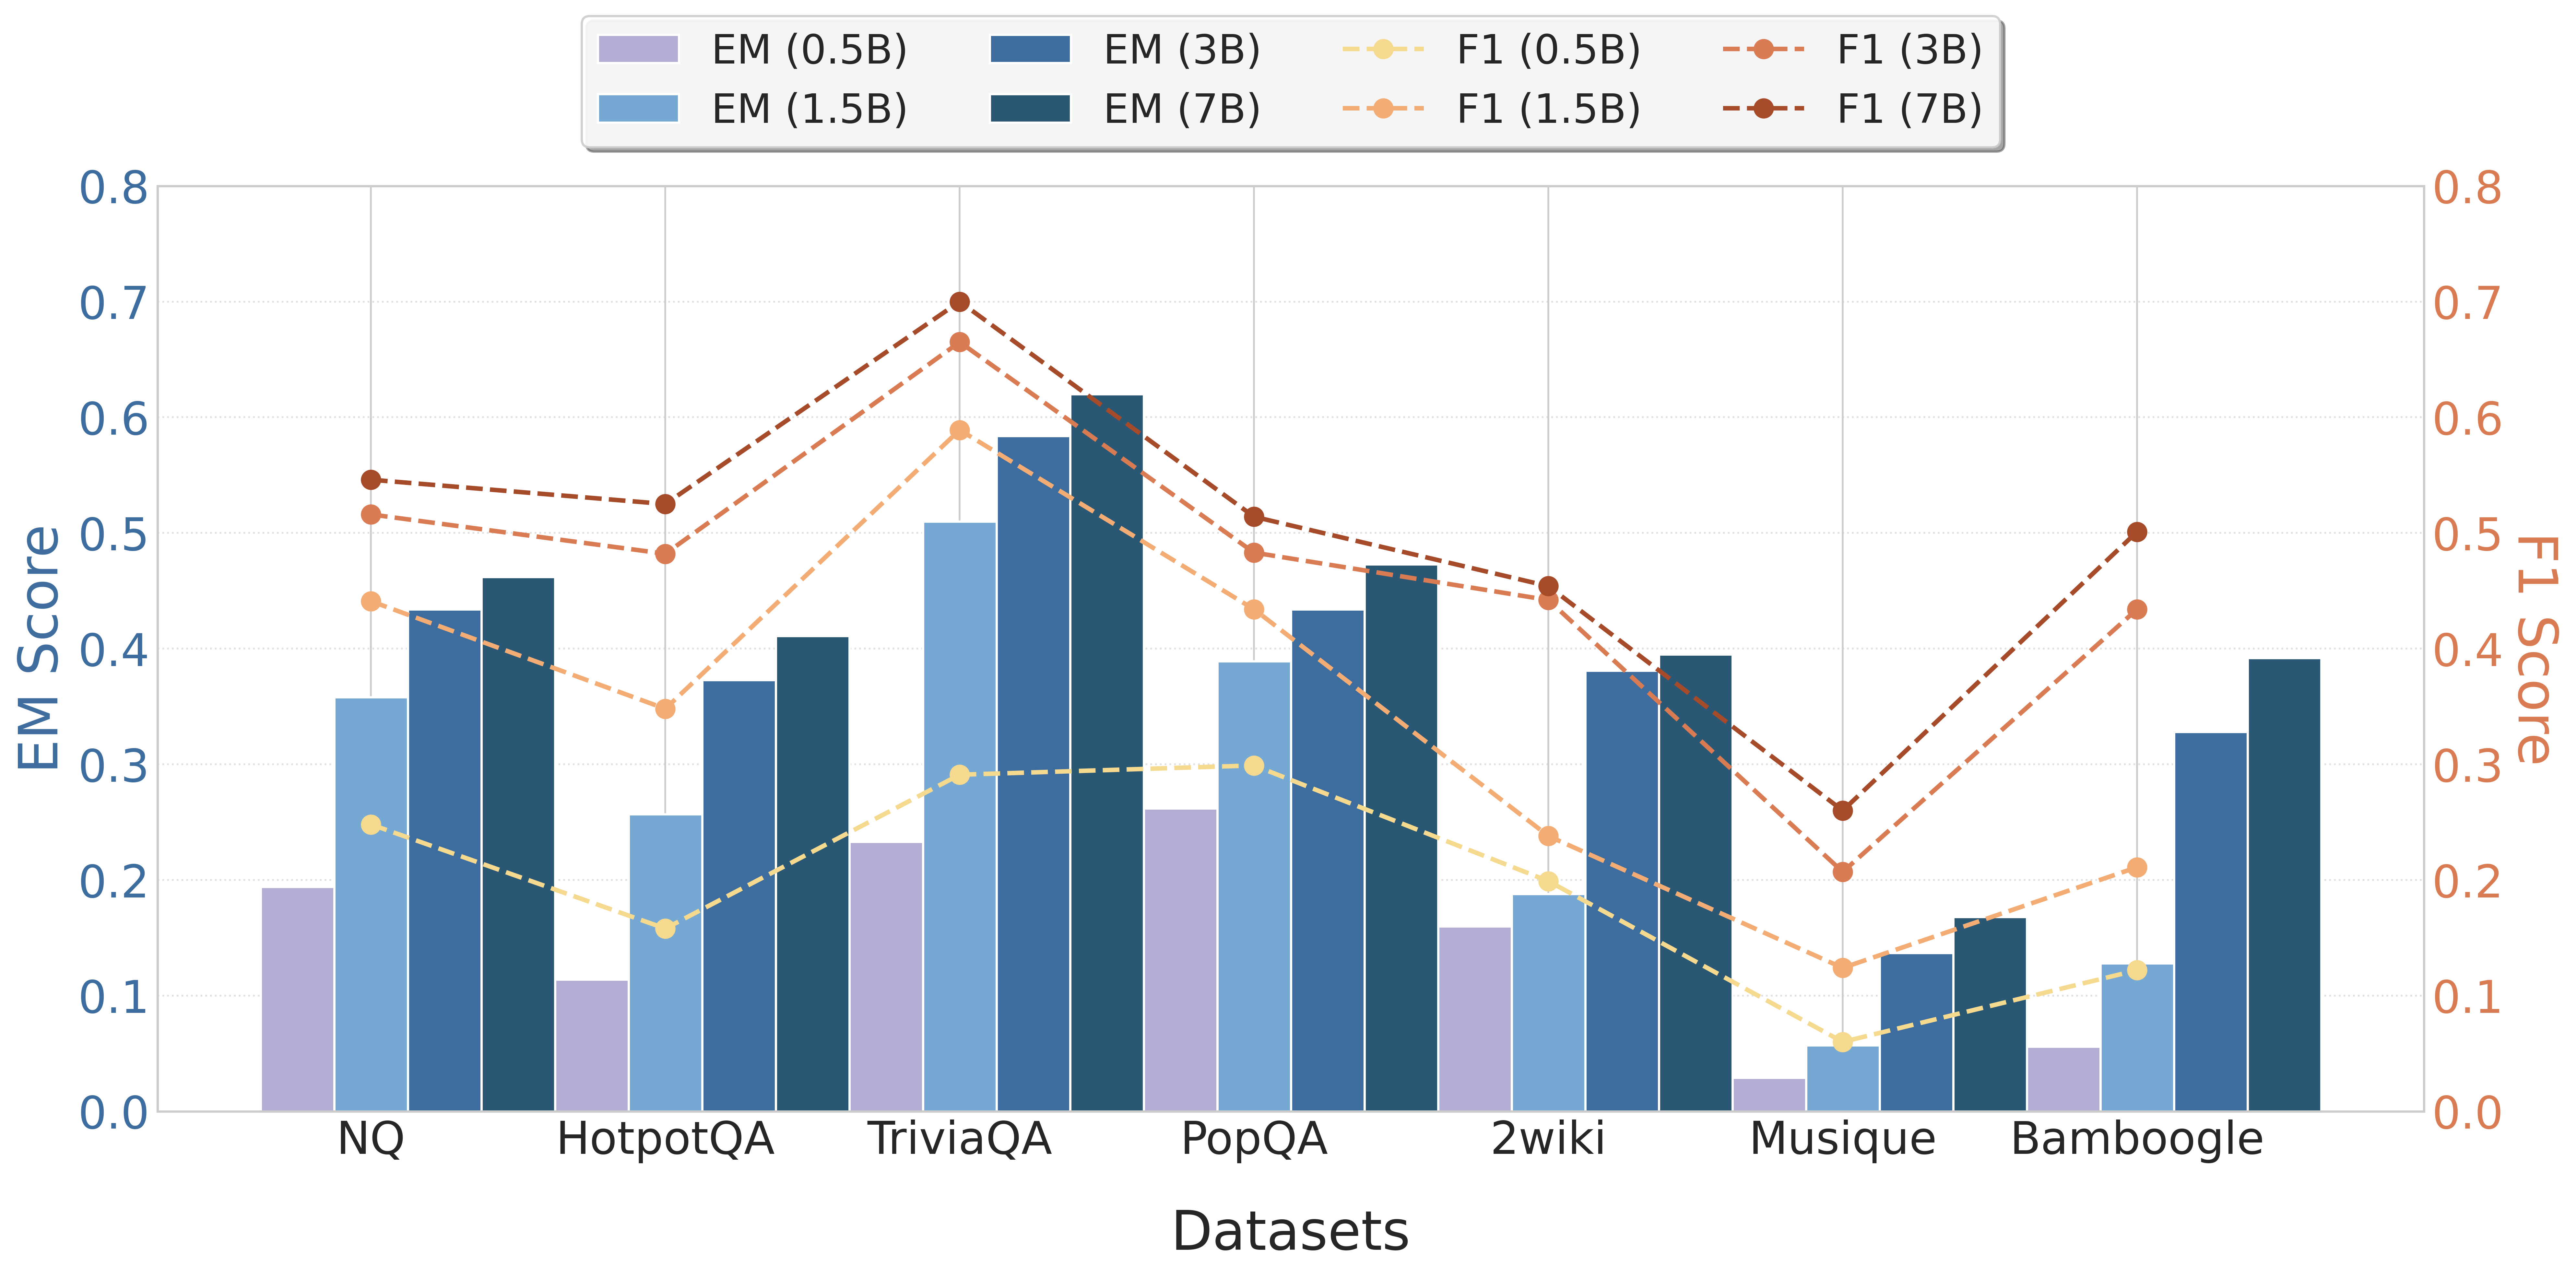
\includegraphics[width=\linewidth]{img/evolver_scaling_results.png}
    \caption{Performance of EvolveR across various model scales.}
    \label{fig:scaling_figure}
\end{wrapfigure}


To validate that our EvolveR framework is a generalizable paradigm rather than a method tailored to a specific model size, we evaluated its performance across a spectrum of open-source model scales. As presented in Figure~\ref{fig:scaling_figure}, we applied EvolveR to Qwen2.5 models of 0.5B, 1.5B, and 3B parameters. The results reveal a clear and consistent positive trend: as the parameter count of the base model increases, the performance of the EvolveR agent improves significantly on every benchmark. The average performance rises monotonically from 0.150 on the 0.5B model to 0.270 on the 1.5B model, and further to 0.382 on the 3B model. This scaling behavior demonstrates that our experience-driven lifecycle effectively harnesses the superior reasoning and instruction-following capabilities inherent in larger foundational models. It confirms that EvolveR acts as a synergistic layer on top of the base model, and suggests that its performance will continue to improve with future advancements in the open-source LLM landscape.



\subsection{Ablation Studies: Dissecting the EvolveR Framework}
\label{sec:ablations}


\subsubsection{Validating the Self-Distillation Mechanism}
A central claim of our work is that an agent can learn effectively through self-distillation. To rigorously investigate this, we compare our standard \texttt{EvolveR (self-distill)} against a strong alternative, \texttt{EvolveR(teacher-distill)}, which uses the powerful GPT-4o-mini as an external model for experience distillation.

The results, presented in Table~\ref{tab:ablation_distill}, reveal a nuanced, scale-dependent relationship. For smaller models like the 0.5B variant, the stronger external teacher provides a clear benefit, as the base model's own distillation capabilities are limited. However, as the model scales to 3B, a reversal occurs: our \texttt{EvolveR (self-distill)} (0.382 avg.) outperforms the teacher-guided variant (0.370 avg.). This is a critical finding, suggesting that as an agent's own reasoning becomes more sophisticated, principles distilled from its own internal policy are ultimately more effective due to better "cognitive alignment". This validates self-distillation as a core, scaling strength of the EvolveR paradigm.



\begin{table*}[t]
    \centering
    \small
    \setlength{\tabcolsep}{1pt}
    \caption{Validating the self-distillation mechanism. We compare our EvolveR, which uses its own model for distillation, against a variant that uses a larger, external model (GPT-4o-mini).}
    \label{tab:ablation_distill}
    \begin{tabular}{l cc ccccc c}
        \toprule
         \multirow{2}{*}{\textbf{Model Variant}} & \multicolumn{2}{c}{\textbf{In domain}} & \multicolumn{5}{c}{\textbf{Out of domain}} & \multirow{2}{*}{\textbf{Avg.}} \\
        \cmidrule(lr){2-3} \cmidrule(lr){4-8}
        & NQ \phup & HotpotQA \phup & TriviaQA \phup & PopQA \phup & 2wiki \phup & Musique \phup & Bamboogle \phup & \\
        \midrule
        \multicolumn{9}{l}{\textbf{Qwen2.5-0.5B}} \\
        EvolveR (self-distill)  & 0.194 \phdown & 0.114 \phup & 0.233 \phup & 0.262 \phup  & 0.160 \phdown & 0.029 \phdown & 0.056 \phdown & 0.150 \phdown \\
        EvolveR (teacher-distill) & 0.281 \up & 0.193 \up & 0.402 \up & 0.363 \up & 0.202 \up & 0.033 \up & 0.064 \up & 0.220 \up \\
        \midrule
        \multicolumn{9}{l}{\textbf{Qwen2.5-1.5B}} \\
        EvolveR (self-distill) & 0.358 \phup & 0.257 \phup & 0.510 \phup & 0.389 \phup & 0.188 \phup & 0.057 \phup & 0.128 \phup & 0.270 \phup \\
        EvolveR (teacher-distill) & 0.352 \down & 0.259  \up & 0.503 \down & 0.395 \up & 0.207 \up & 0.072 \up & 0.240 \up & 0.290 \up \\
        \midrule
        \multicolumn{9}{l}{\textbf{Qwen2.5-3B}} \\
        EvolveR (self-distill) & 0.434 \phup & 0.373 \phup & 0.584 \phup & 0.434 \phup & 0.381 \phup & 0.137 \phup & 0.328 \phup & 0.382 \phup\\
        EvolveR (teacher-distill) & 0.421 \down & 0.372 \down & 0.583 \down & 0.359 \down & 0.437 \up & 0.127 \down & 0.288 \down & 0.370 \down \\
        \bottomrule
    \end{tabular}
\end{table*}



\subsubsection{The Role of Experience Retrieval}
To quantify the direct benefit of providing the agent with access to its distilled principles at inference time. To achieve this, we compare our full \texttt{EvolveR} model against an ablated variant, \texttt{EvolveR w/o exp-retrieve}. It is critical to note that both models undergo the identical experience-driven RL training process. The sole difference is that the \texttt{w/o exp-retrieve} variant is denied access to the experience base during evaluation.

The results in Table~\ref{tab:ablation_retrieval_inference} show a stark performance degradation across all model scales when experience retrieval is disabled. For the 3B model, for instance, the average performance drops significantly from 0.382 to 0.340. This substantial gap underscores a key finding: an agent trained with our EvolveR framework, while powerful on its own, achieves its full potential only when it can access and condition on the relevant principles from its past. This demonstrates that experience retrieval is a critical and indispensable component of the EvolveR paradigm for optimal performance.

\begin{table*}[!ht]
    \centering
    \small
    \setlength{\tabcolsep}{1pt}
    \caption{Investigating the role of experience retrieval at inference time. The \texttt{w/o exp-retrieve} variant uses the same model but is not allowed to access the experience base during evaluation.}
    \label{tab:ablation_retrieval_inference}
    \begin{tabular}{l cc ccccc c}
        \toprule
        \multirow{2}{*}{\textbf{Model Variant}}  & \multicolumn{2}{c}{\textbf{In domain}} & \multicolumn{5}{c}{\textbf{Out of domain}} & \multirow{2}{*}{\textbf{Avg.}} \\
        \cmidrule(lr){2-3} \cmidrule(lr){4-8}
        & NQ \phup & HotpotQA \phup & TriviaQA \phup & PopQA \phup & 2wiki \phup & Musique \phup & Bamboogle \phup & \\
        \midrule
        \multicolumn{9}{l}{\textbf{Qwen2.5-0.5B}} \\
        EvolveR  & 0.194 \phdown & 0.114 \phdown & 0.233 \phdown & 0.262 \phdown & 0.160 \phdown & 0.029 \phdown & 0.056 \phdown & 0.150 \phdown \\
        EvolveR w/o exp-retrieve & 0.085 \down & 0.065 \down & 0.137 \down & 0.150 \down & 0.082 \down & 0.013 \down & 0.016 \down & 0.078 \down \\
        \midrule
        \multicolumn{9}{l}{\textbf{Qwen2.5-1.5B}} \\
        EvolveR & 0.358 \phdown & 0.257 \phdown & 0.510 \phdown & 0.389 \phdown & 0.188 \phdown & 0.057 \phdown & 0.128 \phdown & 0.270 \phdown \\
        EvolveR w/o exp-retrieve & 0.136 \down & 0.112 \down & 0.218 \down & 0.160 \down & 0.136 \down & 0.019 \down & 0.080 \down & 0.123 \down \\
        \midrule
        \multicolumn{9}{l}{\textbf{Qwen2.5-3B}} \\
        EvolveR & 0.434 \phdown & 0.373 \phdown & 0.584 \phdown & 0.434 \phdown & 0.381 & 0.137 \phdown & 0.328 \phdown & 0.382 \phdown \\
        EvolveR w/o exp-retrieve & 0.405 \down  & 0.343 \down & 0.569 \down & 0.392 \down & 0.334 \down & 0.100 \down & 0.240 \down & 0.340 \down \\
        \bottomrule
    \end{tabular}
\end{table*}




\subsubsection{Component-Level Attribution and Memory Configuration}
\label{sec:component_attribution}

To rigorously isolate the contributions of individual components within the EvolveR framework, we systematically ablate principle distillation, experience retrieval and RL. Table~\ref{tab:component_attribution} presents the component-level attribution on the Qwen2.5-3B model. Note that certain component combinations are omitted as they are structurally invalid (e.g., experience retrieval cannot be executed without prior principle distillation).

\begin{table}[ht]
\centering
\caption{Component-level attribution on Qwen2.5-3B.}
\label{tab:component_attribution}
\begin{tabular}{cccc}
\toprule
\textbf{Principle Distillation} & \textbf{Principle Retrieval} & \textbf{RL} & \textbf{Avg. Score} \\
\midrule
No & No & No & 0.134 \\
No & No & Yes & 0.325 \\
Yes & Yes & No & 0.357 \\
Yes & No & Yes & 0.340 \\
Yes & Yes & Yes & \textbf{0.382} \\
\bottomrule
\end{tabular}
\end{table}

The results yield several key observations: First, while RL alone provides a baseline improvement (0.325), it is insufficient to reach optimal performance. Second, experience retrieval contributes a substantial direct gain, improving the RL-only baseline from 0.340 to 0.382. Third, RL further enhances experience-conditioned training, as evidenced by the improvement from the non-RL retrieval setting (0.357) to the full framework (0.382). Overall, principle retrieval and RL act complementarily: retrieval provides the primary reasoning guidance, while RL optimizes the policy to effectively utilize these distilled principles.

To further investigate the role of the experience configuration, we compare different forms of experience construction, as shown in Table~\ref{tab:memory_config}.

\begin{table}[ht]
\centering
\caption{Memory configuration comparison on Qwen2.5-3B.}
\label{tab:memory_config}
\begin{tabular}{ccc}
\toprule
\textbf{Experience Base} & \textbf{Distillation Source} & \textbf{Avg. Score} \\
\midrule
No & None & 0.325 \\
Yes & Teacher-distilled & 0.370 \\
Yes & Self-distilled & \textbf{0.382} \\
\bottomrule
\end{tabular}
\end{table}

This comparison demonstrates that performance gains stem not merely from the presence of a experience base, but fundamentally from how the experience is constructed. Specifically, self-distilled experience outperforms teacher-distilled experience at the 3B scale. This indicates that a experience base aligned with the student model's own policy and specific failure modes provides more actionable and compatible guidance than generic external knowledge.



\subsection{Analysis of Principle Quality and Scalability}
\label{sec:quality_and_scalability}

\textbf{Characterizing Principle Quality and Failure Modes.} 
To systematically evaluate the quality and potential failure modes of the distilled principles, we conducted a manual annotation of 100 sampled principles from the experience base. We categorized them into three mutually exclusive types:

\begin{itemize}[leftmargin=2em]
    \item \textbf{Ideal (Correct \& Actionable):} Logically sound and providing concrete, executable guidance.
    \item \textbf{Vague (Correct but not Actionable):} Logically correct but too generic to effectively guide the model's actions (e.g., ``read the context carefully'').
    \item \textbf{Incorrect / Misleading:} Factually wrong or overly specific/harmful rules that could systematically mislead the reasoning process.
\end{itemize}

We stratified the samples by their assigned metric scores (Low-Score vs. High-Score tiers) to assess the efficacy of our dynamic scoring mechanism.

\begin{table}[ht]
\centering
\caption{Manual annotation of principle quality by score tier.}
\label{tab:principle_quality}
\begin{tabular}{lccc}
\toprule
\textbf{Score Tier} & \textbf{Ideal} & \textbf{Vague} & \textbf{Incorrect / Misleading} \\
\midrule
Low-Score (0.30 - 0.44) & 26\% & 50\% & 24\% \\
High-Score (0.44 - 0.75) & \textbf{82\%} & 10\% & \textbf{8\%} \\
\bottomrule
\end{tabular}
\end{table}

The results in Table~\ref{tab:principle_quality} reveal that the system's primary failure mode in the lower-score tier is the generation of vague advice (50\%) rather than strictly incorrect rules. More importantly, the data confirms that the utility-based scoring-and-pruning mechanism effectively filters out misleading or incorrect principles (reducing them from 24\% to 8\%) while significantly increasing the concentration of highly actionable principles (from 26\% to 82\%).

\textbf{Long-Term Noise Accumulation and Scalability.} 
A critical challenge for experience-augmented agents is the potential for performance degradation and latency bottlenecks as the experience base grows and accumulates noise over time. To investigate the system's robustness to long-term experience expansion, we tracked the Qwen2.5-3B agent's search latency and reasoning performance as the experience base naturally accumulated during training. Evaluations were conducted on a 10\% validation subset randomly sampled across the six benchmarks.

\begin{table}[ht]
\centering
\caption{Scalability dynamics of the experience base.}
\label{tab:scalability}
\begin{tabular}{ccc}
\toprule
\textbf{Experience Base Scale} & \textbf{Top-3 Search Latency} & \textbf{Avg. Score (EM)} \\
\midrule
4,213 & 0.04 s & 0.301 \\
13,435 & 0.06 s & 0.372 \\
23,448 & 0.12 s & 0.382 \\
32,805 & 0.16 s & 0.396 \\
45,083 & 0.19 s & \textbf{0.410} \\
49,934 & 0.20 s & 0.387 \\
\bottomrule
\end{tabular}
\end{table}

As shown in Table~\ref{tab:scalability}, even when the experience base scales to nearly 50,000 principles, the retrieval latency remains negligible (0.20s), indicating that the framework does not face severe computational bottlenecks. Furthermore, despite the massively expanded candidate pool and the inherently increased risk of retrieving noisy principles, the agent's performance does not collapse. Instead, it remains highly stable and peaks at the 45k scale. This provides strong empirical evidence that the combination of semantic deduplication, dynamic scoring, and RL-conditioned policy is highly robust to substantial experience growth and long-term noise.





